\documentclass[
% -- opções da classe memoir --
article,			% indica que é um artigo acadêmico
12pt,				% tamanho da fonte
oneside,			% para impressão apenas no recto. Oposto a twoside
a4paper,			% tamanho do papel. 
english,			% idioma adicional para hifenização
brazil,				% o último idioma é o principal do documento
sumario=tradicional
]{abntex2}
% ---
% PACOTES
% ---
\usepackage{lmodern} % Usa a fonte Latin Modern
\usepackage[T1]{fontenc}% Selecao de codigos de fonte.
\usepackage[utf8]{inputenc}% Codificacao do documento (conversão automática dos acentos)
\usepackage{indentfirst}% Indenta o primeiro parágrafo de cada seção.
\usepackage{nomencl} % Lista de simbolos
\usepackage{color}% Controle das cores
\usepackage{graphicx}% Inclusão de gráficos
\usepackage{microtype}% para melhorias de justificação
\usepackage{gensymb}
\usepackage{caption}
\usepackage{booktabs}

% ---
% Pacotes adicionais, usados apenas no âmbito do Modelo Canônico do abnteX2
% ---
% ---
% Pacotes de citações
% ---
\usepackage[brazilian,hyperpageref]{backref}	 % Paginas com as citações na bibl
%\usepackage[alf,abnt-emphasize=bf]{abntex2cite}	% Citações padrão ABNT
\usepackage[num,overcite,abnt-emphasize=bf]{abntex2cite}	% Citações padrão ABNT
%\citebrackets()
\citebrackets[]
% ---

% ---
% Configurações do pacote backref
% Usado sem a opção hyperpageref de backref
\renewcommand{\backrefpagesname}{Citado na(s) página(s):~}
% Texto padrão antes do número das páginas
\renewcommand{\backref}{}
% Define os textos da citação
\renewcommand*{\backrefalt}[4]{
  \ifcase #1 %
    Nenhuma citação no texto.%
    \or
    Citado na página #2.%
  \else
    Citado nas páginas #2.%
\fi}%
% ---

\graphicspath{{./images/} {/home/victor/Pictures/latex/}}

% --- Informações de dados para CAPA e FOLHA DE ROSTO ---
\titulo{\bfseries Sistemas Embarcados e suas aplicações na agricultura IOT: revisão bibliográfica}
\tituloestrangeiro{Embedded Systems and their applications in agriculture IOT: bibliographic review}

%\autor{Victor Emanuel Almeida}
\autor{
  %UNIOESTE\thanks{``Universidade Estadual do Oeste do Paraná, Foz do Iguaçu, Brasil.'' \url{http://www.unioeste.br/}} 
  %\\[0.5cm]\\
  Victor Emanuel Almeida\thanks{``Estudante de Ciência da Computação na Universidade Estadual do Oeste do Paraná (UNIOESTE), campus de Foz do Iguaçu-PR, Brasil.''\url{http://www.unioeste.br/}}
}

\local{FOZ DO IGUAÇU}
\data{\today}

\instituicao{%
\par
Universidade do Oeste do Paraná 
\par
UNIOESTE
}
\instituicao{Curso de Ciência da Computação, da Universidade Estadual do Oeste do Paraná (UNIOESTE), Campus Foz do Iguaçu-PR, Brasil}

\preambulo{Escrever Preâmbulo}

\tipotrabalho{Trabalho Acadêmico}
% ---

% ---
% Configurações de aparência do PDF final

% alterando o aspecto da cor azul
\definecolor{blue}{RGB}{41,5,195}

% informações do PDF
\makeatletter
\hypersetup{
  %pagebackref=true,
  pdftitle={\@title}, 
  pdfauthor={\@author},
  pdfsubject={software livre},
  pdfcreator={\@author},
  pdfkeywords={software livre},
  colorlinks=true,% false: boxed links; true: colored links
  linkcolor=black,% color of internal links
  citecolor=blue,% color of links to bibliography
  filecolor=magenta,% color of file links
  urlcolor=blue,
  bookmarksdepth=4
}
\makeatother
% --- 

% ---
% compila o indice
% ---
\makeindex
% ---

% ---
% Altera as margens padrões
% ---
\setlrmarginsandblock{3cm}{2cm}{*}
\setulmarginsandblock{3cm}{2cm}{*}
\checkandfixthelayout
% ---

% --- 
% Espaçamentos entre linhas e parágrafos 
% --- 

% O tamanho do parágrafo é dado por:
\setlength{\parindent}{1.25cm}
%\setlength{\parindent}{1.5\lineheight}

% Controle do espaçamento entre um parágrafo e outro:
%\setlength{\parskip}{0.2cm}  % tente também \onelineskip
\setlength{\parskip}{\onelineskip}

% Espaçamento simples
\SingleSpacing

% ----
% Início do documento
% ----
\begin{document}
%\pagenumbering{roman}
% Seleciona o idioma do documento (conforme pacotes do babel)
%\selectlanguage{english}
\selectlanguage{brazil}

% Retira espaço extra obsoleto entre as frases.
\frenchspacing 

% ----------------------------------------------------------
% ELEMENTOS PRÉ-TEXTUAIS
% ----------------------------------------------------------

%---
%
% Se desejar escrever o artigo em duas colunas, descomente a linha abaixo
% e a linha com o texto ``FIM DE ARTIGO EM DUAS COLUNAS''.
%\twocolumn[    		% INICIO DE ARTIGO EM DUAS COLUNAS
%
%---

% página de titulo principal (obrigatório)
%\imprimircapa
%\begin{center}
\maketitle
%{\centered\maketitle\imprimirlocal\imprimirinstituicao}
%\imprimirtitulo
%\vspace{.5cm}

%\imprimirinstituicao
%\end{center}

% titulo em outro idioma (opcional)

% resumo em português
\begin{resumoumacoluna}
  Escrever resumo

  \textbf{Palavras-chave}: Agricultura, Internet das coisas, Tomada de decisão, Sensoreamento.

  \vspace{\onelineskip}

  \noindent
\end{resumoumacoluna}


% resumo em inglês
\renewcommand{\resumoname}{Abstract}
\begin{resumoumacoluna}
  \begin{otherlanguage*}{english}
    Escrever resumo
    \vspace{\onelineskip}
    \noindent

    \textbf {Keywords}: Agriculture, Internet of things, Decision making, Sensing.
  \end{otherlanguage*}  
\end{resumoumacoluna}

%\cleardoublepage
%\pdfbookmark[0]{\contentsname}{toc}
%\tableofcontents*
%\cleardoublepage
%\listoffigures
%\cleardoublepage
%\listoftables

%]  				% FIM DE ARTIGO EM DUAS COLUNAS
% ---

% ----------------------------------------------------------
% ELEMENTOS TEXTUAIS
% ----------------------------------------------------------
\textual
%\setcounter{page}{1}
%\pagenumbering{arabic}
% ----------------------------------------------------------
% Introdução
% ----------------------------------------------------------
\section{Introdução}

Introduzir o assunto de IOT, terminando com citação

Mostrar a relevância da pesquisa, como verificar o que o mundo tem feito deve nos mostrar as melhores práticas bem como as últimas tecnologias disponíveis.

\section{Conceitos e características (Mudar nome)}\label{Conceitos Importantes}
Antes de abordar as principais tecnologias, bem como os principais e mais atuais estudos relacionados a IOT, faz-se necessário elucidar alguns pontos.
\subsection{O que é IOT}\label{O que é IOT}

O termo \textit{Internet of Things (IOT)}, em português internet das coisas foi elaborado pelo britânico, Kevin Ashton, em 1999\cite{5} e se refere de forma geral a uma rede que conecta diversas ``coisas'' a internet, através de software, com o objetivo de trocar informações\cite{defIot}, tais ``coisas'' podem ser sensores, microcontroladores ou até mesmo objetos que nunca imaginamos tais como geladeiras, televisores, entre outros.

\subsection{Por que usar IOT na agricultura}\label{Por que usar IOT na agricultura}
Segundo \citeauthor{5} A agricultura é um dos setores que deve ser altamente influenciado pela internet das coisas pela necessidade de eficiência na gestão de recursos bem como o amadurecimento do conceito da agricultura de precisão, \textit{Precision agriculture}\cite{PrecisionAg}, que seria a arte e ciência de usar tecnologia avançada para aumentar a produção agrícola\cite{9}, a qual necessita das últimas tecnologias da área somado a muita computação para obter medições não invasivas em tempo real de forma rápida, precisa e confiável de diversas variáveis como (monitoramento do solo, do ar, da água, das plantas, dos animais, da irrigação\ldots)\cite{10} e para obter previsões apoiando assim a tomada de decisão, tais previsões serão abordadas na seção~\ref{Plataformas de tomada de decisão} e as medições precisas e confiáveis na seção~\ref{Sensoreamento do solo (camada de percepção)}.

Outro fator importante que torna o setor agrícola tão favorável ao uso de internet das coisas é por serem grandes áreas que precisam de constante monitoramento e controle, nas palavras de \citeauthor{10} esses fatores o torna ``candidatos ideais''.

\subsection{As camadas do IOT}\label{As camadas do IOT}

  Estrutura do IOT: baseada em três camadas\cite{5} principais bem como uma camada intermediária:
    \begin{enumerate}
      \item A de percepção que seria uma camada de sensores, hardware, que obtém-se dados relevantes a respeito dos fenômenos meteorológicos tais como clima, temperatura do solo, umidade do ar, entre outros.
      \item A camada de comunicação, camada a qual é responsável por enviar os dados coletados pela camada de percepção supracitada para servidores ou aplicações na nuvem, de forma geral para algum tipo de armazenamento. Possuindo diversos protocolos de comunicação tais como \textbf{Ipv4} e \textbf{Ipv6}\cite{camada2}.
      \item A de aplicação, camada a qual trás sentido aos dados coletados pelos sensores, pois é nesse momento que ocorre o processamento dos dados, nessa revisão bibliográfica essa camada será responsável principalmente por mostrar ao agricultor informações relevantes de forma simples e compreensível, bem como informá-lo qual o melhor momento para plantar\cite{1}, ou em quais lugares da plantação tem doenças\cite{2}.
      \item Midleware camada intermediária a qual
    \end{enumerate}

\section{Materiais e Métodos}\label{Materiais e Métodos}
Perguntar


\begin{table}[!htb]
  \centering
  \caption{Palavras chaves que se repetem}
  \begin{tabular}{|c|l|}
    \hline
    \textbf{Ocorrências} & \textbf{Palavra(s) chave} \\ \hline
    4                    & wireless sensor           \\ \hline
    4                    & precision agriculture     \\ \hline
    4                    & internet of things        \\ \hline
    4                    & sensor network            \\ \hline
    2                    & soil moisture             \\ \hline
    2                    & precision viticulture     \\ \hline
  \end{tabular}
\end{table}

\begin{table}[!htb]
  \centering
  \caption{Ano de publicação dos artigos Qualis A}
  \begin{tabular}{|c|c|}
    \hline
    \textbf{Ano de publicação} & \textbf{Quantidade de artigos} \\ \hline
    2008 & 1 \\ \hline
    2014 & 1 \\ \hline
    2015 & 2 \\ \hline
    2016 & 1 \\ \hline
    2017 & 4 \\ \hline
    2018 & 1 \\ \hline
    2019 & 3 \\ \hline
  \end{tabular}
\end{table}

%\begin{figure}[!htb]
  %\centering
  %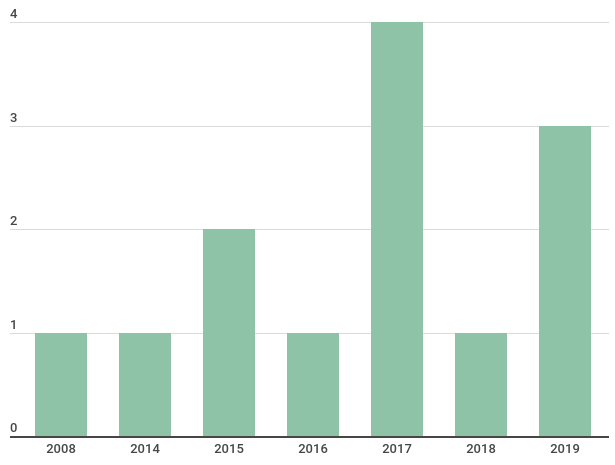
\includegraphics[width=\textwidth]{artigosA.png}
  %\caption{\label{fig:artigosA.png}Ano de publicação dos artigos Qualis A}
%\end{figure}
%
%\begin{figure}[!htb]
  %\centering
  %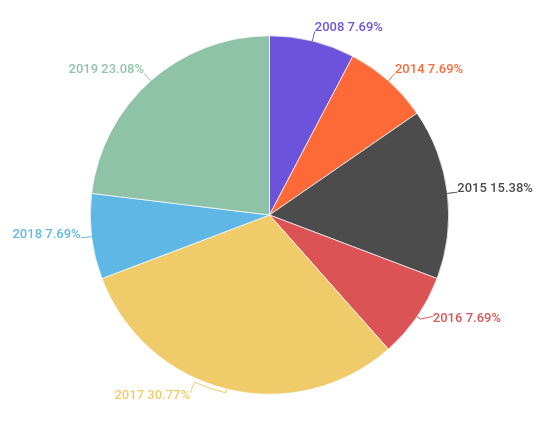
\includegraphics[width=\textwidth]{artigosA_pizza.png}
  %\caption{\label{fig:artigosA_pizza.png}Ano de publicação dos artigos Qualis A}
%\end{figure}


\section{Sensoreamento (camada de percepção)}\label{Sensoreamento do solo (camada de percepção)}

Tendo em vista a vasta variabilidade dos sensores utilizados nas diversas pesquisas apresentadas, agregamos os melhores resultados a cerca dos sensores.

\subsection{Umidade do solo}\label{Umidade do solo}

A umidade do solo se refere à água presente na parte superior de um solo\cite{11}

também falar que pode ser medido em outras profundidades do solo como no caso de \citeauthor{12}

A literatura sobre a umidade do solo é muito extensa e está se
desenvolvendo tão rapidamente que pode ser considerado ambicioso buscar apresentar o estado da arte no que diz respeito à pesquisa dessa variável-chave\cite{11}

, e segundo~\citeauthor{3}, os métodos mais aceitos para medição da umidade do solo são \textit{time domain reflectometry (TDR)} em português reflectometria no domínio do tempo e os métodos que medem a capacitância, sendo esses utilizados pela maioria dos sensores modernos.

Analisando esses sensores o autor supracitado\cite{3} realizou diversos testes alterando parâmetros como salinidade do solo, condutividade elétrica, temperatura entre outros, com os sensores EC-5 e ECH$_2$O-TE, chegando a seguinte conclusão, que medições realizadas a uma frequência de 70 MHz obtém-se dados expressivos, sendo essa a frequência mais eficiente, pois acima dela o gasto energético  e eletrônico não resultam em maior precisão. Sendo assim para cada sensor deve ser achado a frequência ideal de medição na qual o custo é minimizado e a precisão é aumentada.

Esses sensores de umidade que medem a capacitância apesar de seguirem o mesmo principio de funcionamento, podem variar muito de preço e precisão por exemplo o caso seja necessário uma elevada precisão bem como outros dados tais como salinidade e temperatura será utilizado um sensor mais caro como o utilizado por \citeauthor{12} para medições precisas o suficiente para agendar irrigação por gotejamento, tais medições foram feitas com 2 sensores Hydra probes, um a 15 cm de profundidade e outro medindo desses 15 cm até a superficie.

Como já comentado no parágrafo anterior variam muito de preço e funcionalidades. Sendo assim não existe um sensor perfeito ou universal para todo tipo de projeto, dessa maneira faz-se necessário que se avalie o orçamento bem como as funcionalidades e precisão exigidas, para auxiliar nisso criamos a tabela abaixo

\begin{table}[!htb]
  \centering
  \caption{Comparando sensores de umidade do solo}
  \begin{tabular}{lllll}
    \hline
    \textbf{Sensor} & \textbf{Preco} & \textbf{Temperatura} & \textbf{Salinidade} & \textbf{Umidade} \\ \hline
    Hydra Probe     & 440 - 800 RS   & $\pm~1$\textdegree C & Mede                & Mede             \\
                    &                &                      &                     &                  \\
                    &                &                      &                     &                 
  \end{tabular}
\end{table}

\section{Rede (camada de comunicação)}\label{Rede (camada de comunicação)}

\section{Plataformas de tomada de decisão (camada de aplicação)}\label{Plataformas de tomada de decisão}

Apesar de existir iniciativas que visem plataformas de tomada de decisão mais universais e interoperáveis tais como o mySense\cite{7} e o SenseTube\cite{6}. A maioria das plataformas de tomada de decisão abaixo tendem a resolver um único problema específico ou servem apenas para pesquisas

%que facilitem a criação de interfaces com o usuário final bem como a calibração de sensores

%Explicar como cada plataforma de tomada de decisão é diferente e cada autor decide implementar da sua maneira, apesar de ter esforços para padronizações\cite{6}



Em relação às plataformas de tomada de decisão segundo a pesquisa de~\citeauthor{1} até onde sabe-se no ano de~\citeyear{1} não havia nenhuma plataforma ou \textit{framework} que baseando-se na temperatura do solo fornecesse dados dinâmicos para informar em tempo real decisões agronômicas dependentes do solo, tal como momento do plantio, irrigação entre outros.

Considerando essa lacuna do conhecimento, desenvolveu-se uma ferramenta de suporte à decisão da temperatura do solo, ``\textit{temperature decision support tool}'', seguindo uma metodologia de cinco passos:
\begin{enumerate}
  \item Comparação dos dados climáticos e ambientais, conseguindo a variabilidade em larga escala da temperatura do solo.

  \item Comparação das temperaturas médias em séries históricas.
  \item Comparar variáveis preditoras de clima com as medições realizadas, obtendo previsões.
  \item Transformar o sistema para funcionar em tempo real.
  \item Investigações a longo prazo.
\end{enumerate}

Com o objetivo de aumentar a precisão utiliza-se nove variáveis preditoras de clima, sendo elas: temperatura máxima, radiação diária, diferença entre temperatura máxima e mínima, taxa pluviométrica, latitude, elevação, conteúdo de água do solo, difusão térmica do solo, dia do ano.

Este sistema foi desenvolvido em Shiny (R), e possui uma alta taxa de predição de 92\% de validação cruzada R$_{2}$, RMSE = 1,91, tendência percentual = $-$ 0,01.
Com essas taxas de predição pode-se auxiliar os agricultores de algodão a realizarem o plantio no momento certo, classificando o solo como ``bom'' após três dias com temperaturas acima de 14\textdegree C, dessa maneira após utilizar dados de variáveis preditoras supracitadas recomenda-se ou não o plantio.

Outro sistema de apoio à decisão desenvolvido por~\citeauthor{2}, com o objetivo de monitorar vinhedos para encontrar e tratar ``míldio'' (mofo).
O míldio é uma doença fúngica causada pela \textit{plasmopara viticola oomycete}, doença essa que causa muito prejuízo nas vinícolas\cite{2}. Doença essa muito estudada, sendo assim nessa pesquisa baseando-se nos modelos já existentes de detecção a acompanhamento do fungo, buscou-se a automatização dos mesmos.

O principal modelo utilizado para descobrir qual o momento mais propício de aparecimento do míldio foi o de Goidanich\cite{detectando_milidio}, também chamado de ``regra dos três dez'' pois quando a temperatura média ultrapassa 10\textdegree C, a germinação ultrapassa os 10 cm e o volume de chuva superior a 10 mm, este é o momento propício para uma primeira contaminação da vinha.
Sabendo desses dados expostos por Goidanich\cite{detectando_milidio} percebe-se a necessidade de monitorar três fenômenos, sendo eles: temperatura, umidade e índice pluviométrico, sendo assim precisando de três sensores.

Para desenvolver essa plataforma o autor utilizou o sistema ``\textit{Sense Our Environment}'' (SEnviro), uma plataforma que utilizando-se de software e hardware livres visa baixar o custo e aumentar a eficiência energética dos sensores\cite{2}. O SEnviro contém suas funcionalidades melhor explicado em outra pesquisa\cite{SEnviro} e como já citado nessa seção possui todos os códigos fonte disponível ao público no github\cite{SEnviro_Github}.


Com a estação concluída iniciou-se os testes, detectando em 96,9\% de maneira precisa em que houve o alerta de infecções. Através disso, os agricultores puderam aplicar o tratamento de controle de praga apenas quando necessário, reduzindo assim a quantidade de produtos químicos no solo, a quantidade de horas gastas para verificação e correção de doenças dentro do vinhedo bem como os custos da plantação.

\section{Considerações Finais}

% ----------------------------------------------------------
% ELEMENTOS PÓS-TEXTUAIS
% ----------------------------------------------------------
\postextual

% ----------------------------------------------------------
% Referências bibliográficas
% ----------------------------------------------------------
\cleardoublepage
\bibliography{ref}

% ----------------------------------------------------------
% Glossário
% ----------------------------------------------------------
%
% Há diversas soluções prontas para glossário em LaTeX. 
% Consulte o manual do abnTeX2 para obter sugestões.
%
%\glossary

\end{document}
